\documentclass[runningheads]{llncs}



% All the packages etc.
\usepackage{xspace}
\usepackage{todonotes}
\usepackage{amsmath}
\usepackage[hidelinks]{hyperref}
\usepackage{cleveref}



\usepackage[edges]{forest}

\usepackage{tikz}
\usepackage{tikzscale}
\usetikzlibrary{positioning, shapes.multipart, arrows.meta, backgrounds, fit, quotes}
\tikzstyle{myborder}=[densely dashed]



\newcommand{\dlfont}[1]{\ensuremath{\mathsf{#1}}}

\newcommand{\riskman}{\textsc{Riskman}\xspace}
\newcommand{\eqdef}{\mathrel{:=}}

\newcommand{\ind}[1]{\dlfont{#1}}
\newcommand{\indid}[2]{$\dlfont{#1}_{\dlfont{#2}}$}
\newcommand{\indidb}[2]{(\indid{#1}{#2})}
\newcommand{\indb}[1]{(\ind{#1})}

\newcommand{\vdespec}{VDE Spec 90025\xspace}
\newcommand{\metadata}[2]{\textbf{#1}: #2}




% Springer-style cref
\crefname{section}{Sect.}{Sect.}
\Crefname{section}{Sect.}{Sect.}
\crefname{figure}{Fig.}{Fig.}
\Crefname{figure}{Fig.}{Fig.}


\title{Safe Design Arguments (SDAs) -- tips ane examples}

\author{%
      Piotr Gorczyca\inst{1}\orcidID{0000-0002-6613-6061} \and
      Dörthe Arndt\inst{1}\orcidID{0000-0002-7401-8487} \and
      Martin Diller\inst{2}\orcidID{0000-0001-6342-0756} \and
      Pascal Kettmann\inst{1}\orcidID{0009-0009-9461-7952} \and
      Stephan Mennicke\inst{3}\orcidID{0000-0002-3293-2940} \and
      Hannes~Strass\inst{1}\orcidID{0000-0001-6180-6452}
}
%
\authorrunning{P.~Gorczyca et al.}
% First names are abbreviated in the running head.
% If there are more than two authors, 'et al.' is used.
%
\institute{%
      Computational Logic Group, Institute of Artificial Intelligence \and
      Logic Programming and Argumentation Group, Institute of Artificial Intelligence \and
      Knowledge-Based Systems Group, Institute for Theoretical Computer Science\\
      \inst{1,2,3}~Faculty of Computer Science, TU Dresden, Germany\\
      \email{\ttfamily firstname.lastname@tu-dresden.de}
}



\begin{document}



\maketitle


\begin{tabular}{l}
    \metadata{Documentation}{\url{https://w3id.org/riskman/}}    \\
    \metadata{Ontology}{\url{https://w3id.org/riskman/ontology}} \\
    \metadata{Shapes}{\url{https://w3id.org/riskman/shapes}}     \\
    \metadata{GitHub repository}{\url{https://w3id.org/riskman/repo}}
\end{tabular}





\section{SDAs}


The central notion of the \riskman ontology \& shapes is that of a \emph{Safe Design Argument} (SDA), which is a building block of the so-called SDA trees. SDA trees can be seen as simplifications of \emph{Assurance Cases} (ACs)~\cite{WeinstockG09}, in that they also represent structures of measures mitigating certain risk, but the AC notions (such as e.g. \emph{claim}, \emph{strategy}, \emph{evidence} or \emph{instantiation}) are by design built into the SDAs. SDAs by being uniform building blocks help to avoid the complexity of modelling risk mitigation strategies using AC approach.

SDAs allow to conceal concrete and potentially manufacturer-sensitive data by capturing only the abstract idea of risk mitigation. That enables their transparency and reusability: these abstract ideas are expected to reside in an open source repository from which they could be pulled by manufacturers whenever needed. Popular SDA would gain credability through frequent implementation (and hence certification) which would in turn hopefully lead to a so-called \emph{safety competition}: a state in which SDAs addressing the same risk are competing to be recognized as the safest.

For a concrete risk management file submission an abstract idea is not enough: it is necessary to provide the details of implementation of the SDA within the device as well as the evidence of the implementation. This requirement is realized by means of an \emph{Implementation Manifest}, which is a piece of information supplied to an SDA containing the aforementioned information. An SDA containing an Implementation Manifest is called a \emph{Safe Design Argument Implementation} (SDAI).

SDA (SDAI) is the base, abstract superclass of \emph{Risk SDA} (\emph{Risk SDAI}) and \emph{Assurance SDA} (\emph{Assurance SDAI}), the two SDA subclasses to be used in practice. Whenever given SDA is referring to some state of the art \emph{Safety Assurance} -- e.g. a section of a norm or standard mentioning a particular way of handling a risk, we speak about the latter -- Assurance SDA(I). Otherwise, in the case of the absence of the Safety Assurance, we are dealing with Risk SDA(I).

As an example, consider a scenario in which a risk of electrocution appears and, as prevention, the manufacturer decides to use electrical insulation. The concrete value of distance through insulation has been decided to be 0.5mm.
The structure of a corresponding Risk SDA is depicted below:

  \[
    \underbrace{
      \overbrace{\text{ Electrical insulation }}^{\textit{ Risk SDA }}
      |
      \overbrace{\text{ dist=0.5mm }}^{\textit{Impl. manifest}}
    }_\textit{Risk SDAI}
  \]

On the other hand, assume that the manufacturer is aware that in their scenario (under adequate assumptions), a mitigation specified in IEC 60601-1~\footnote{IEC 60601 is a series of technical standards published by the International Electrotechnical Commission, addressing safety aspect of medical electronical devices.} is applicable, which further specifies the insulation distance to be at least 0.4mm. In this case the manufacturer could refer to the respective clause of IEC 60601-1 (clause 8.8.2) as the Safety Assurance of the related SDA. The structure of such Assurance SDA is shown below:
\[
\underbrace{
    \overbrace{\text{ Electrical insulation }
    |
    \overbrace{\text{ IEC 60601-1, s 8.8: min. dist.}>0.4\text{mm}}^{\textit{Safety Assurance}}}^{\textit{Assurance SDA}}
    |
    \overbrace{\text{dist=0.5mm }}^{\textit{Impl. Manifest}}
}_\textit{Assurance  SDAI}
\]


The above example illustrates the difference between Risk- and Assurance SDA(I)s. An additional reference to a state-of-the-art measure in a form of a Safety Assurance can help in establishing SDAs credability and traceability in case of an unforeseen event.

The hierarchical relation between an SDAs similar to that known from AC, in that the children SDAs jointly realize the goal/claim of its parent.  
The \riskman approach additionally imposes the two following constraints on the structure of SDA trees: 
\begin{enumerate}
  \item all children nodes of Assurance SDA(I)s must again be Assurance SDA(I)s,
  \item all leaf nodes must have an Implementation Manifest (effectively, must be SDAIs).
\end{enumerate}

\noindent~Non-leaf nodes may have Implementation Manifests, but it is not strictly required. 


\section{Insulin infusion pump example}
\emph{Insulin infusion pumps}
%a paradigmatic example for assurance cases in risk management~\cite{FDA14}\todo{MD\&HS@MD: add further citations}, 
aid in regulating blood glucose levels, especially of patients with diabetes, by administering fast-acting insulin via a catheter inserted beneath the skin. Based on the risk assessment for a generic infusion pump by Zhang et al.~\cite{zhangJJ10,zhangJJR11}, \Cref{fig:rmf} shows %data about 
a controlled risk and associated SDA that can be extracted from a risk management file that follows \vdespec.%

Following~Zhang et al.~\cite[entry 4.3.9 in Table 4 in the appendix]{zhangJJ10}, the risk stems from a ``non-audio alarm malfunction'' hazard (with associated id \ind{hz} in the figure).
Specifically, the vibration mechanism of the non-audio alarm integrated into the pump may fail (event \indid{ev}{1}).
Then, the patient may not become aware of an issue (event \indid{ev}{2}), which can lead to the patient receiving less insulin (hazardous situation \ind{hs}) and the patient losing consciousness (harm \ind{hr}).
Apart from the information for the domain specific hazard \indb{dsh} required by VDE Spec (dashed boxes in the figure exemplarily group related elements), the \riskman ontology also allows to refer to terminology for medical device problems put forward by the International Medical Device Regulators Forum (IMDRF)~\cite{IMDRF20AET} (field with id \ind{dp}).
The SDA (\indid{sd}{0}, based on the work of Zhang et al.~\cite[Table 3]{zhangJJR11}) consists of three sub-SDAs and expresses that there are alternative means of alerting the patient.
The first sub-SDA \indidb{sd}{1} specifically expresses that the alarm condition is also indicated through visual signals.
Moreover, the second sub-SDA \indidb{sd}{2} indicates that this notification is recurring.
The third SDA \indidb{sd}{3} expresses that there is also an additional audio alarm that will start unless the patient acknowledges the vibration or blinking.
Moreover, according to sub-SDA \indidb{sd}{5} the audible signal is in accordance with regulations, here the assurance is IEC 60601 \indb{sa}. Thus, sub-SDA \indidb{sd}{5} is the only assurance SDA (indicated by the pink colour); all other SDAs are risk SDAs (purple).
On the other hand, as required by VDE Spec, each leaf SDA is an SDAI, with the associated implementation manifests (\indid{im}{1},\indid{im}{2},\indid{im}{4},\indid{im}{5}) pointing to implementation details and documentation.
\begin{figure}[]
    \centering
    \resizebox{1\textwidth}{!}{
        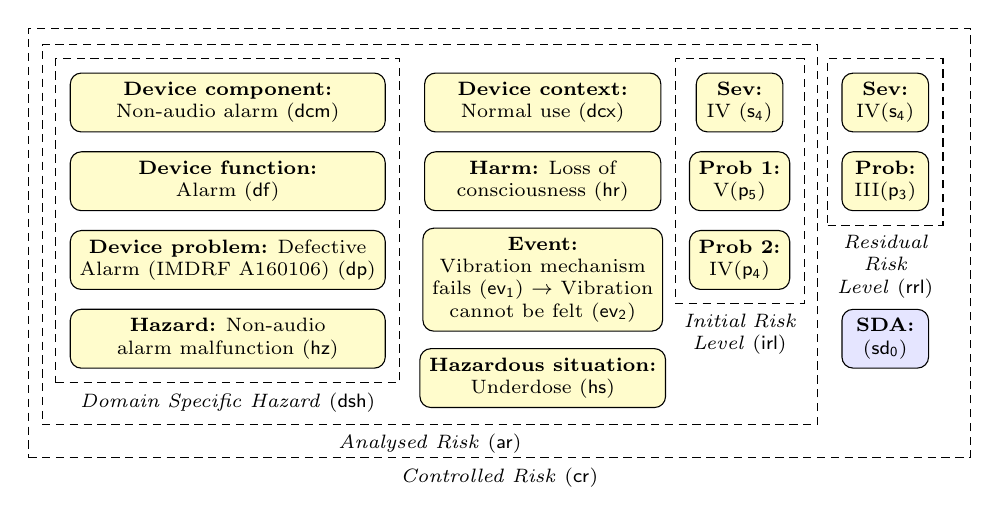
\begin{tikzpicture}
            \tikzset {
                basic node/.style={
                        draw,
                        % text width=1cm,
                        font=\scriptsize,
                        align=center,
                        rounded corners,
                        minimum width=1.1cm,
                        fill=yellow!20
                    }}

            % DSH    
            \node[basic node, minimum width=4cm] (dcomponent) at (0,0) {\textbf{Device component:}\\Non-audio alarm \indb{dcm}};
            \node[basic node, minimum width=4cm] (dfunction) at (0,-1) {\textbf{Device function:}\\Alarm \indb{df}};
            \node[basic node, minimum width=4cm] (dfunction) at (0,-2) {\textbf{Device problem:} Defective\\Alarm (IMDRF A160106) \indb{dp}};
            \node[basic node, minimum width=4cm] (hazard) at (0,-3) {\textbf{Hazard:} Non-audio \\alarm malfunction \indb{hz}};

            % 
            \node[basic node, minimum width=3cm] (dcontext) at (4,0) {\textbf{Device context:}\\Normal use \indb{dcx}};
            \node[basic node, minimum width=3cm] (harm) at (4,-1) {\textbf{Harm:} Loss of\\consciousness \indb{hr}};
            \node[basic node, minimum width=3cm] (event) at (4,-2.25) {\textbf{Event:}\\Vibration mechanism\\fails \indidb{ev}{1} $\rightarrow$ Vibration\\cannot be felt \indidb{ev}{2}};
            \node[basic node, minimum width=3cm] (hazsit) at (4,-3.5) {\textbf{Hazardous situation:}\\Underdose \indb{hs}};

            % IRL
            \node[basic node] (sev) at (6.5,0) {\textbf{Sev:}\\IV \indidb{s}{4}};
            \node[basic node] (prob1) at (6.5,-1) {\textbf{Prob 1:}\\V\indidb{p}{5}};
            \node[basic node] (prob2) at (6.5,-2) {\textbf{Prob 2:}\\IV\indidb{p}{4}};

            % IRL
            \node[basic node] (rsev) at (8.35,0) {\textbf{Sev:}\\IV\indidb{s}{4}};
            \node[basic node] (rprob) at (8.35,-1) {\textbf{Prob:}\\III\indidb{p}{3}};

            \node[basic node, fill=blue!10] (sda0) at (8.35,-3) {\textbf{SDA:}\\\indidb{sd}{0}};

            % DSH
            \node[draw,myborder,fit=(dcomponent)(dfunction)(hazard),inner sep=5pt,label={[font=\scriptsize]south:\textit{Domain Specific Hazard}~\indb{dsh}}] {};
            % IRL
            \node[draw,myborder,fit=(sev)(prob1)(prob2),inner sep=5pt,label={[font=\scriptsize, text width=1.5cm, align=center]south:\textit{Initial Risk Level}~\indb{irl}}] {};
            % RRL
            \node[draw,myborder,fit=(rsev)(rprob),inner sep=5pt,label={[font=\scriptsize, text width=1.5cm, align=center]south:\textit{Residual Risk Level}~\indb{rrl}}] {};
            % ARisk
            \node[draw,myborder,fit=(dcomponent)(hazard)(prob2),inner xsep=10pt, inner ysep=15pt, yshift=-5pt, label={[font=\scriptsize]south:\textit{Analysed Risk}~\indb{ar}}] {};
            % CRisk
            \node[draw,myborder,fit=(dcomponent)(sda0),inner xsep=15pt, inner ysep=24pt, yshift=-8pt, label={[font=\scriptsize]south:\textit{Controlled Risk}~\indb{cr}}] {};
        \end{tikzpicture}}%
    \\\resizebox{1\textwidth}{!}{
        \begin{forest}
            forked edges,
            for tree={align=center,base=bottom,draw,font=\scriptsize,edge={->},rounded corners,scale=0.9},
            im/.style={fill=green!10},
            sa/.style={fill=purple!15},
            sda/.style={fill=blue!10},
            asda/.style={fill=brown!15},
            [\textbf{SDA}:\\Alternative alerting when vibration mechanism of non-audio alarm fails~\indidb{sd}{0}, sda,
            [\textbf{SDA}:Additional\\visual (blinking)\\signal \indidb{sd}{1},sda,name=sda1
            [\textbf{IM}: Sec. 10.3 \\ of Alarm\\report \indidb{im}{1},im,name=im1]],
            [\textbf{SDA}: Notification\\ recurs every\\ $X$ minutes \indidb{sd}{2},sda,name=sda2
            [{\textbf{IM}: $X\eqdef 0.5$, \\ Sec. 10.7 \\ of Alarm\\report \indidb{im}{2}},im]],
            [\textbf{SDA}: Additio-\\nal audio\\alarm \indidb{sd}{3},sda,name=asda3
            [\textbf{SDA}: Audio\\signal if vibration\\signal not\\acknowledged \indidb{sd}{4},sda,name=asda4
            [\textbf{IM}: Sec. \\ 10.11  of Alarm\\report \indidb{im}{4},im]],
            [\textbf{SDA}:\\Audible signal is\\at least X db \\ at Y m  \indidb{sd}{5},asda,name=asda5
            [{\textbf{IM}:  $X\eqdef 45$, \\ $Y\eqdef 1$ ,  Sec. 5.3 \\ of  Loudspeaker \\ test \indidb{im}{5}},im,name=im5]],
            [\textbf{SA}: IEC\\60601 \indb{sa}, no edge, sa,name=sa5,yshift=6pt]
            ],
            ]
            \draw[->] (asda5) to (sa5);
            \node[draw,myborder,fit=(sda1)(im1),label={[font=\scriptsize]south:\textit{SDAI}}] {};
            \node[draw,myborder,fit=(asda5)(sa5),label={[font=\scriptsize, text width=1.8cm, xshift=25pt, align=right]south:\textit{Assurance SDA}}] {};
            \node[draw,myborder,fit=(asda5)(sa5)(im5),inner sep=5pt,label={[font=\scriptsize]south:\textit{Assurance SDAI}}] {};
        \end{forest}
    }
    \caption{Graphical representation of the data of a controlled risk (top figure) and associated SDA (bottom figure) provided within a risk management file for an infusion pump. The dashed indicate  examples of composite classes, e.g. \indidb{sd}{1} and \indidb{im}{1} together constitute an SDAI. Note that these are just single examples of SDAIs, as any pair of an SDA and its related Implementation Manifest jointly realize an SDAI, e.g. the pair \indidb{sd}{2} + \indidb{im}{2} or \indidb{sd}{4} + \indidb{im}{4}. 
    }
    \label{fig:rmf}
\end{figure}


\bibliographystyle{splncs04}
\bibliography{bib/references}

\end{document}


